\documentclass{article}
\usepackage{tikz}
\usepackage{amsmath}
\usepackage{graphicx}
\usepackage{float} % for [H] specifier

\begin{document}

\section*{Enchufes y Adaptadores}

En la próxima cumbre internacional de cuestiones importantes se recibirán periodistas de todo el mundo en un hotel que antaño era moderno pero hoy es simplemente lujoso y antiguo. Como antes no se usaban muchos artefactos eléctricos, solo algunos tomacorrientes de cada tipo fueron instalados en la sala de la cumbre. El tiempo pasó y los artefactos eléctricos se empezaron a utilizar mucho más, además de que surgieron nuevos tipos de tomacorrientes. Antes de que comience la cumbre, se recolectó la información de los dispositivos que van a traer los periodistas para adquirir los adaptadores necesarios, los cuales se comprarán en un fabricante particular. Cada adaptador de este fabricante tiene una forma de entrada y una forma de salida. Estos adaptadores se pueden encadenar tanto como se quiera, lo cual es bueno porque la fábrica no vende todos los tipos de adaptadores existentes. Por suerte, sí tienen la posibilidad de fabricar una cantidad ilimitada de los adaptadores que venden.

\begin{enumerate}
    \item Proponer un modelo de flujo para minimizar la cantidad de dispositivos que se quedan sin corriente eléctrica sabiendo:
    \begin{itemize}
        \item que los periodistas traerán $d_i$ dispositivos que usan un tomacorrientes de cada tipo $i$,
        \item que la sala principal tiene $t_i$ tomacorrientes de cada tipo $i$,
        \item cuáles son los pares $ij$ de entradas y salida de los adaptadores vendidos por la fábrica.
    \end{itemize}
    
    \item Dar una interpretación a cada unidad de flujo y cada restricción de capacidad.
    
    \item Determinar la complejidad de resolver el modelo resultante con el algoritmo de Edmonds y Karp.
\end{enumerate}

Planteamos el siguiente modelo de grafo: Tenemos una sola "columna" de vértices, numerados del $1$ hasta $n$. Cada vértice $v_i$ representa un tipo de enchufe. Conectamos cada vértice $v_i$ a una fuente $s$, con capacidad $d_i$, y a un sumidero $t$ con capacidad $t_i$. Las conexiones entre dos vértices $(v_i,v_j)$ existen si y solo si el adaptador $(i,j)$ es manufacturado por la fábrica.

\begin{figure}[H]

\begin{center}
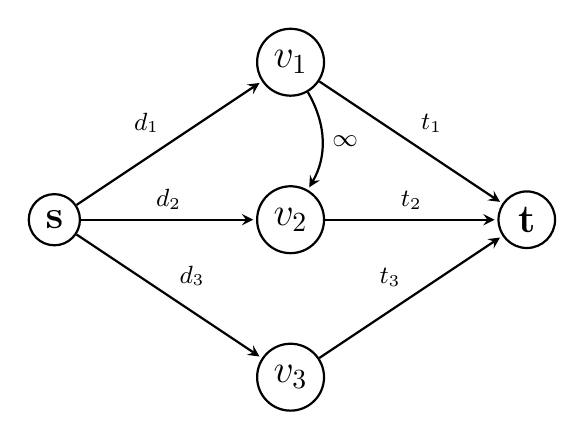
\begin{tikzpicture}[->,>=stealth,shorten >=1pt,auto,node distance=3cm,
                    thick,main node/.style={circle,draw,font=\Large\bfseries}]

  \node[main node] (s) at (0,0) {s};
  \node[main node] (v1) at (3,2) {$v_1$};
  \node[main node] (v2) at (3,0) {$v_2$};
  \node[main node] (v3) at (3,-2) {$v_3$};
  \node[main node] (t) at (6,0) {t};

  \path[every node/.style={font=\sffamily\small}]
    (s) edge node {$d_1$} (v1)
        edge node {$d_2$} (v2)
        edge node {$d_3$} (v3)
    (v1) edge node {$t_1$} (t)
    (v2) edge node {$t_2$} (t)
    (v3) edge node {$t_3$} (t)
    (v1) edge[bend left] node {$\infty$} (v2); % Infinite capacity edge

\end{tikzpicture}
\end{center}
\caption{Ejemplo con adaptador (1,2)}
\end{figure}


\textbf{Interpretación del flujo:} Dado un flujo máximo, sabemos que el flujo pasando por las aristas que interconectan a los nodos distintos de $s$ y $t$, representa la cantidad de adaptadores necesarios de ese tipo. El flujo máximo será la cantidad de dispositivos que pudimos conectar exitosamente. La capacidad que va de cada arista $v_i$ a la fuente es la cantidad de aparatos que (ya sea que usen adaptador o no) se conectan a los tomacorrientes de tipo $i$.

\textbf{Complejidad:} $|V| = n + 2$, $|E| = 2n + \#$adaptadores. El flujo máximo no tiene cota, depende de los valores de $t_i$ y $d_i$.

El algoritmo de Edmonds-Karp tiene una complejidad de $O(\min(|V| \cdot |E|^2, |V| \cdot F)) = O(\min(n \cdot (2n + \#$adaptadores$)^2, n \cdot F))$.


\end{document}
